\documentclass[../report.tex]{subfiles}

\begin{document}

\par Nous souhaitons désormais estimer les quantiles extrêmes de la distribution de températures, notre objectif étant de déterminer le "risque de canicule" entre le 15 juillet et le 15 aout à Bordeaux.


\subsection{Méthodologie}

% Données.
\par Nous conservons la même base de données que dans la partie précédente, mais nous considérons dans cette partie les mesures de températures maximales journalières prises entre le 15 juillet et le 15 août de chaque année, afin d'effacer le caractère saisonnier mis en évidence dans la première partie. Nous faisons l'approximation - peut-être grossière - que ces valeurs sont indépendantes. Rappelons que les températures sont fournies sous l'unité 10 * \SI{}{\celsius}.

% Contexte.
\par Nous supposons ainsi que ces données correspondent à $n$ observations i.i.d. $X_1, ..., X_n$ d'une loi $\mathbb{P}$ inconnue. L'objectif est d'estimer, pour $\alpha \in \left[0, 1 \right]$ proche de 1, le quantile d'ordre $\alpha$ de cette loi. Cela nous donnera la valeur de température qui ne sera pas dépassée - avec un niveau de confiance $\alpha$. Notre mesure de "risque de canicule" sera alors la valeur de $\alpha$ pour laquelle cette température maximale est \SI{35}{\celsius}.

% Méthode.
\par Pour cela, comme mis en évidence dans le cours, nous ne considérons pas de méthodes de type paramétriques ou de quantiles empiriques, mais préférons une approche par domaine d'attraction. Nous supposons ainsi que $X_1, ..., X_n$ sont dans le domaine d'attraction d'une certaine loi max-stable, ce qui d'après le cours implique l'existence de $\xi \in \mathbb{R}$ caractérisant cette loi max-stable sous la forme
\begin{displaymath}
H_{\xi} = 
	\begin{cases}
	e^{- {\left( 1 + \xi x \right)}^{-\frac{1}{\xi}}} &\text{si } \xi \neq 0 \\
	e^{-e^{-x}} &\text{si } \xi = 0
	\end{cases}
\end{displaymath}

\par La première chose est de déterminer une estimation du paramètre $\xi$, ce que nous faisons dans la section suivante. Nous tâcherons ensuite de proposer une estimation du quantile désiré.

% Vérification des résultats.
\par En revanche, il est difficile de chercher à vérifier les résultats, sachant que nous ne connaissons pas la loi exacte de $X_1$. Il est donc difficile de proposer un test statistique de vérification, et les résultats que nous obtenons restent spéculatifs.


\subsection{Estimation de $\xi$}
\par Au lieu d'appliquer aveuglément des calculs d'estimateurs à nos données, étudions-les. Nous pouvons représenter graphiquement les valeurs de températures : 
\begin{figure}[H]
  \centering
    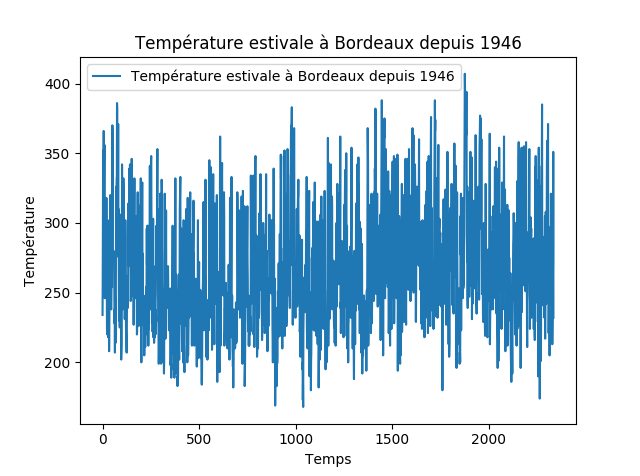
\includegraphics[width=0.7\textwidth]{images/part_2/temperatures.png}
  \caption{Données}
\end{figure}

\par Nous constatons que les données présentent une grande variance, et qu'il y a peu d'événements extrêmes. Pour confirmer cette impression, nous traçons le diagramme quantile-quantile des données, comparant la distribution de celles-ci avec celle de la loi normale :

\begin{figure}[H]
  \centering
    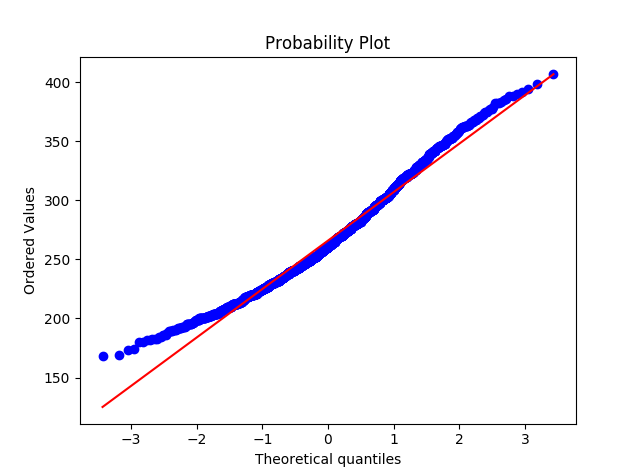
\includegraphics[width=0.7\textwidth]{images/part_2/qqplot.png}
  \caption{Diagramme quantile-quantile}
\end{figure}

\par Nous remarquons une asymétrie des queues de distribution : la queue de distribution correspondant aux valeurs extrêmes négatives est épaisse, mais celle correspondant aux valeurs extrêmes positives est relativement fine. Ainsi, les événements extrêmes les plus récurrents sont ceux de faibles températures et non de forte températures. Or notre problématique est celle des canicules, ce qui signifie que la loi que nous considérons n'est pas une loi à queue de distribution forte. Nous nous attendons donc heuristiquement à une valeur de $\xi$ négative, puisque nous savons que les lois $H_{\xi}$ pour $\xi > 0$ correspondent sont \emph{heavy-tailed}.

\par NB : Nous constatons un phénomène symétrique lorsque nous étudions les températures minimales en hiver : dans ce cas ce sont les occurrences de températures chaudes qui sont plus récurrentes que les températures froides.

\par Nous devons donc adapter les méthodes du cours puisque celles-ci correspondaient à $\xi > 0$. Notamment, nous ne pouvons pas utiliser l'estimateur de Hill.

\par Comme mentionné dans le cours, nous pouvons en revanche dans cette situation utiliser l'estimateur de Pickands :
\begin{equation}
  \tag{Estimateur de Pickands}
  \hat{\xi}_{n, k \left( n \right)}^{P} = \frac{1}{\log \left( 2 \right)} \log \left( \frac{ X_{\left( n - k \left( n \right) + 1, n\right)} - X_{\left( n - 2 k \left( n \right) + 1, n\right)}}{X_{\left( n - 2 k \left( n \right) + 1, n\right)} - X_{\left( n - 4 k \left( n \right) + 1, n\right)}} \right)
\end{equation}

où $X_{\left(i, n \right)}$ correspond à la i-ème plus grande valeur parmi tous les $X_j$.

\par Des résultats théoriques montrent que l'estimateur converge en probabilités vers la vraie valeur sous les conditions 
\begin{displaymath}
	\begin{cases}
	k \left( n \right) &\xrightarrow[n \to + \infty]{} + \infty \\
	\frac{k \left( n \right)}{n} &\xrightarrow[n \to + \infty]{} 0
	\end{cases}
\end{displaymath}

\par Il s'agit donc de trouver un compromis entre la valeur de $k$ et celle de $n$. En pratique, nous traçons le graphe de $ \hat{\xi}_{n, k \left( n \right)}$ en fonction de $k$ (la valeur de $n$ est fixée et correspond au nombre d'observations), et nous cherchons une "zone de stabilité" correspondant à la valeur estimée de $\xi$. Nous obtenons le graphe suivant : 
\begin{figure}[H]
  \centering
    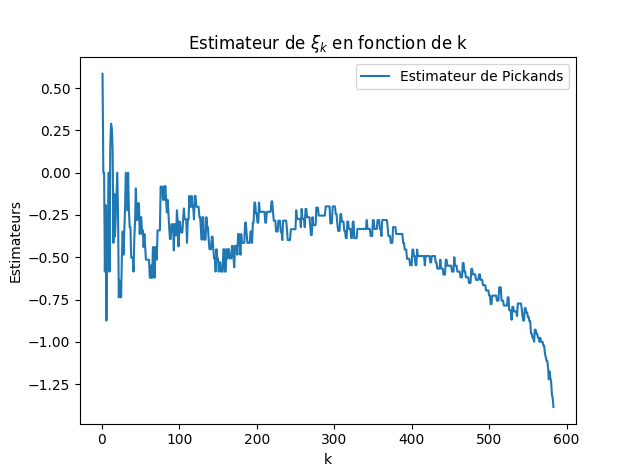
\includegraphics[width=0.7\textwidth]{images/part_2/pickands.png}
  \caption{Diagramme quantile-quantile}
\end{figure}

\par Nous pouvons constater que, comme prédit par l'analyse heuristique précédente des données, cette méthode propose un estimateur négatif. Nous observons un domaine de stabilité pour $k \in \left[ 200; 400 \right]$ et nous pouvons choisir pour valeur de $\xi$ l'estimation associée :
\begin{displaymath}
\hat{\xi} = -0.3
\end{displaymath}
\par Notons qu'en vertu des résultats du cours, le fait que $\xi$ soit négatif implique l'existence d'une constante $x_F$ telle que pour $x \geq x_F$, $\mathbb{P} \left( X \geq x \right) = 1$. L'interprétation physique de la canicule pourrait confirmer ce phénomène, mais l'existence d'un tel $x_F$ rend difficile et moins pertinentes les analyses de risque.

\par Nous ne pouvons donc pas exploiter le fait que - selon un théorème vu en cours - il existe une fonction $L$ à variations lentes telle que la fonction de répartition voulue s'écrive
\begin{displaymath}
\bar{F} \left( x_F - \frac{1}{x} \right) = x^{\frac{1}{\xi}} L \left( x \right)
\end{displaymath}

puisque nous ne savons pas estimer $x_F$. Nous allons devoir employer une autre approche.


\subsection{Méthode \emph{peak over threshold}}
\par Rappelons l'algorithme de la méthode \emph{peak over threshold} présentée durant le cours. 
\par Dans un premier temps, nous estimons $u > 0$ tel que la fonction empirique $e_n$ définie par 
\begin{displaymath}
e_n \left( x \right) := \frac{1}{N_x} \sum\limits_{i, X_i > x} \left( X_i - x \right)
\end{displaymath}
( ù $N_u : = card \left\lbrace i \in \left[ 1; n \right], X_i > u \right\rbrace$), soit à peu près linéaire pour $x \geq u$.
\par Nous notons ensuite $Y_i := X_i - u$ les excès, et nous calculons (numériquement) $\hat{\xi} \in \mathbb{R}$ et $\hat{\beta} > 0$ maximisant le maximum de vraisemblance 
\begin{displaymath}
L = - n \log \left( \beta \right) - \left( \frac{1}{\xi} + 1 \right) \sum\limits_{i = 1}^n \log \left( 1 + \frac{\xi Y_i}{\beta} \right)
\end{displaymath}
\par Alors pour tout $y > 0$, nous pouvons estimer la fonction de répartition recherchée par 
\begin{displaymath}
\hat{\bar{F}} \left( u + y \right) = \frac{N_u}{n} {\left( 1 + \frac{\hat{\xi} y}{\hat{\beta}} \right)}^{-\frac{1}{\hat{\xi}}}
\end{displaymath}

\par Nous traçons d'abord le graphe de $e_n \left( x \right)$ en fonction de la température $x$ et obtenons :
\begin{figure}[H]
  \centering
    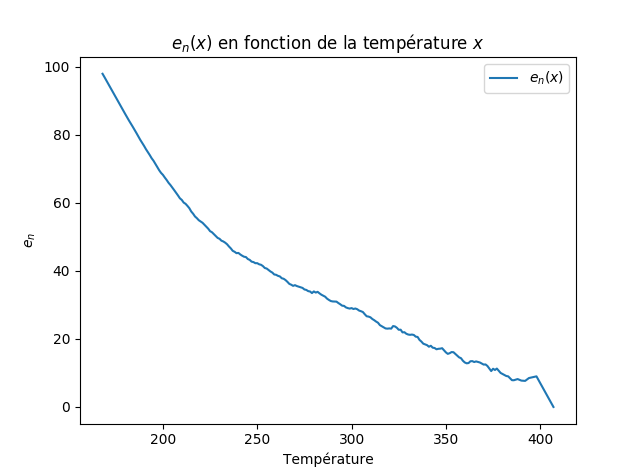
\includegraphics[width=0.7\textwidth]{images/part_2/e_n.png}
  \caption{Graphe de $e_n$}
\end{figure}

\par Nous observons que la croissance semble être quadratique dans un premier temps, puis linéaire à partir de $u = 225$. Nous conservons cette valeur de $u$ et réalisons numériquement l'optimisation de la vraisemblance. Nous trouvons 
\begin{displaymath}
\begin{cases}
\hat{\xi} &= -0.764\\
\hat{\beta} &= 150
\end{cases}
\end{displaymath}

\par Cela semble bien confirmer le phénomène établi dans la section précédente d'une fine queue de distribution.

\par Estimant $\xi$ et $\beta$ par régression linéaire sur la fonction $e_n \left( u \right) \simeq \frac{\beta + \xi u}{1 - \xi}$, nous obtenons des résultats ayant le même ordre de grandeur : 
\begin{displaymath}
\begin{cases}
\hat{\xi} &= -0.376\\
\hat{\beta} &= 152
\end{cases}
\end{displaymath}

\par Nous pouvons dès lors tracer la fonction de répartition estimée selon les deux méthodes, que nous comparons avec la fonction de répartition empirique :
\begin{figure}[H]
  \centering
    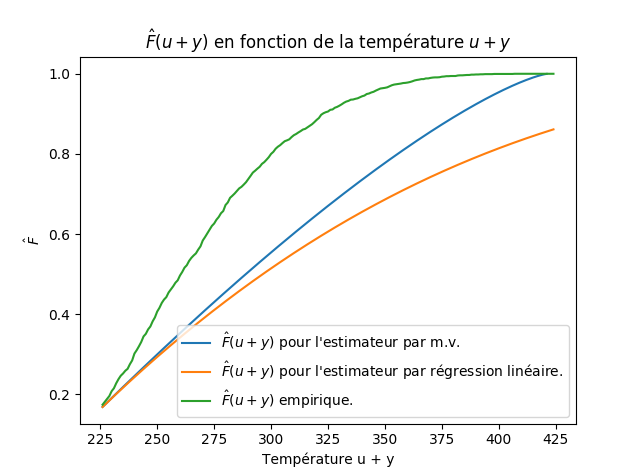
\includegraphics[width=0.7\textwidth]{images/part_2/repartition.png}
  \caption{Fonctions de répartition}
\end{figure}

\par Malheureusement, les résultats ne sont pas très pertinents, car les fonctions estimées n'approximent pas très bien la fonction de répartition empirique, même si ils restent relativement consistants avec le fait que la queue de distribution observée est fine. Réalisant l'application numérique, nous trouvons
\begin{displaymath}
\mathbb{P} \left( X \geq \SI{35}{\celsius} \right) = 
	\begin{cases}
	0.78 \quad &\text{pour l'estimateur du maximum de vraisemblance} \\
	0.69 \quad &\text{pour l'estimateur par régression linéaire} \\
	0.96 \quad &\text{pour l'estimateur empirique} \\
	\end{cases}
\end{displaymath}

\par Ainsi les modèles proposés, même si ils respectent le fait que la queue de distribution soit fine, ne permettent pas d'obtenir des résultats précis pour des événements rares. On peut en revanche imaginer qu'ils sont plus pertinents pour les événements très rares car on constate que l'estimateur du maximum de vraisemblance semble devenir proche de l'estimateur empirique pour des températures supérieures à \SI{41}{\celsius}.

\end{document}